\subsection{Impedance Conversion} \label{subsec:SeriesToParallel}
The $\bar v$ and $\bar i$ signals described in section \refq{sec:ImpedanceAnalysis} can be used to characterize the DUT, but the signals say nothing about how the impedance is supposed to be modelled. The impedance of a DUT could have the form shown on figure \refq{fig:4_1_5_DUTXSeriesParallel} where the DUT has a series resistance $R_s$ in series with a parallel connection of a pure reactance $X$, from either a capacitor or inductor, and a parallel resistor $R_p$. Both $R_s$ and $R_p$ cause power dissipation in the DUT. The value $R_s$ is also known as \textit{equivalent series resistance}, or ESR:

\begin{figure}[H]
    \centering
    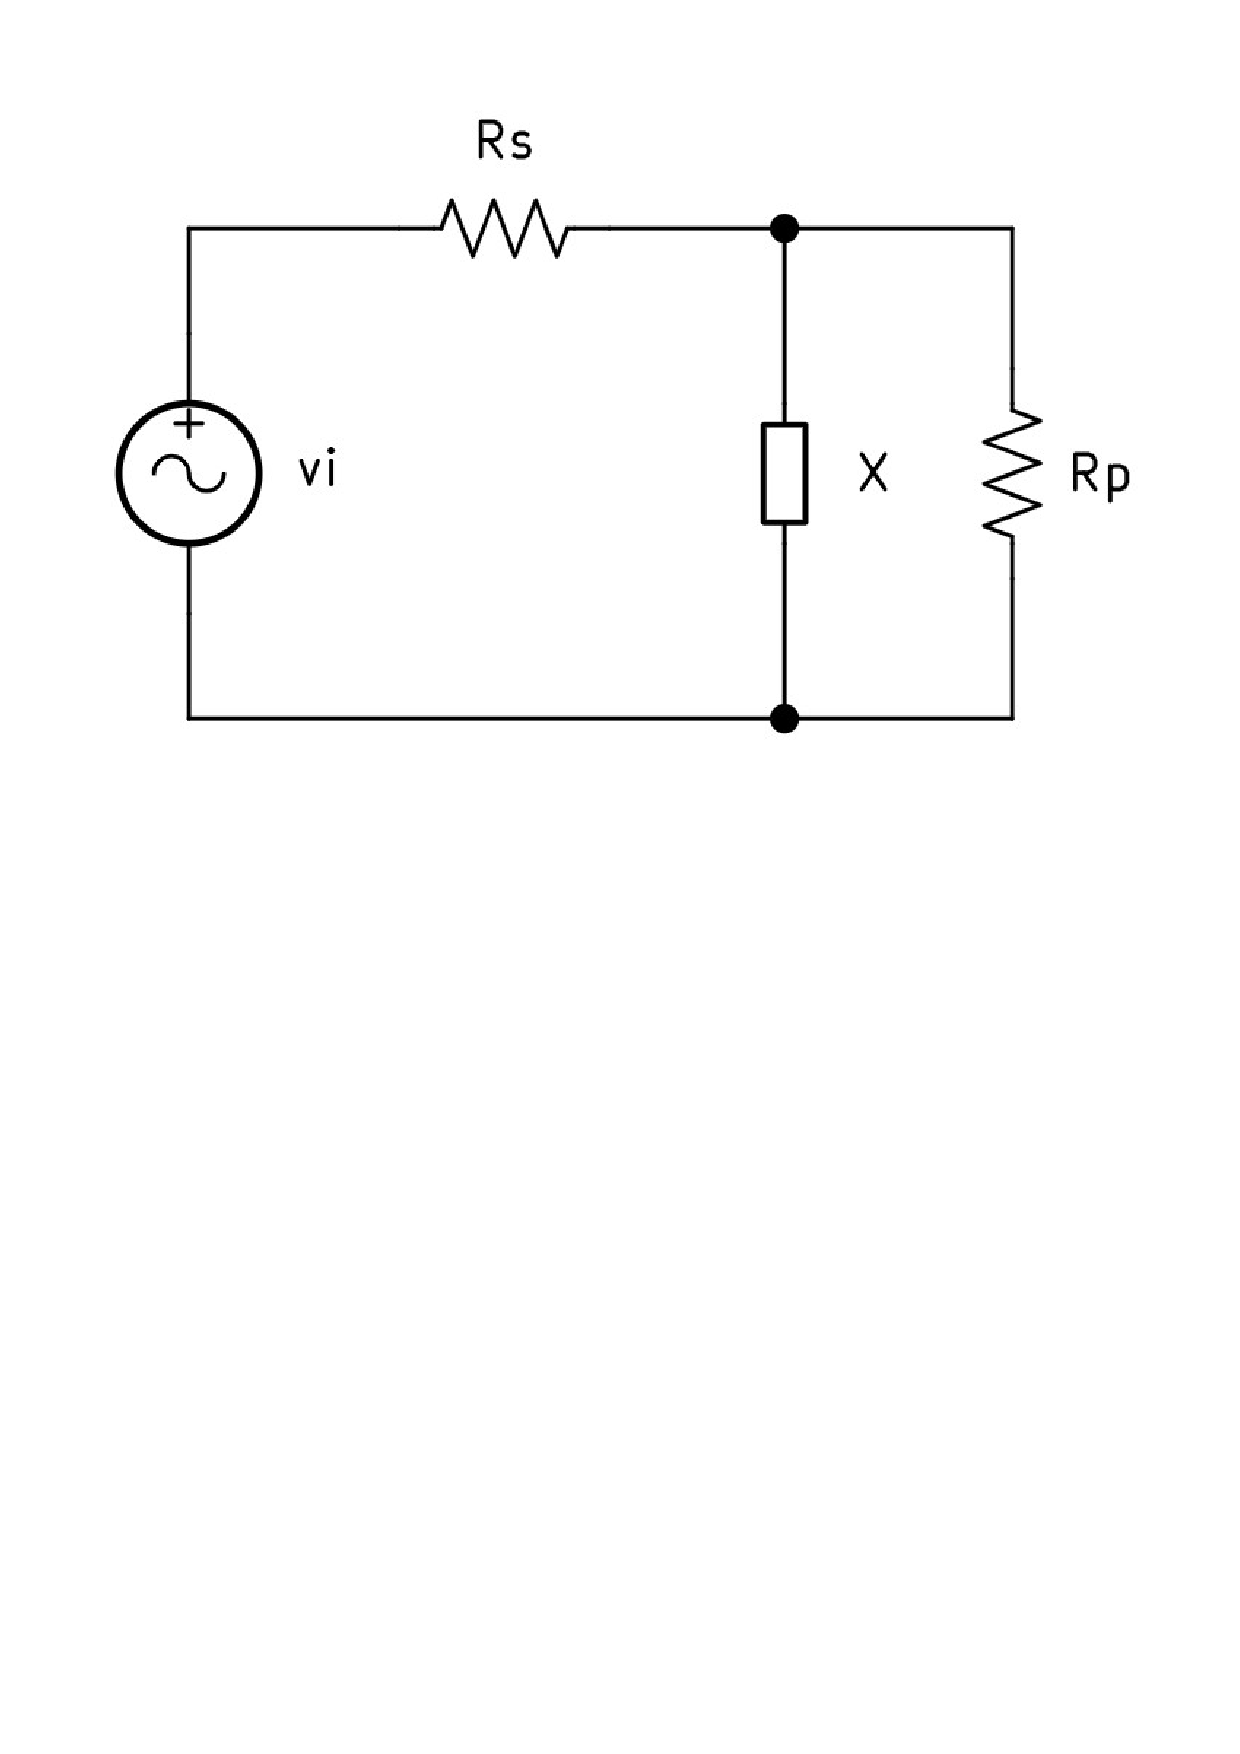
\includegraphics[clip, trim=0 450 0 0, width=0.4\textwidth]{Sections/4_TechnicalAnalysis/Figures/4_1_1_DUTXSeriesParallel.pdf}
    \caption{A simple model of a DUT. The pure reactance X has a series resistance and a parallel resistance.}
    \label{fig:4_1_5_DUTXSeriesParallel}
\end{figure}

If the reactance on figure \refq{fig:4_1_5_DUTXSeriesParallel} is a capacitor then then parallel resistance $R_p$ will, typically, be a large value while the series resistance $R_s$ is small. Eq \refq{eq:4_1_1_CapCurrent5} in section \refq{subsec:Reactance} states that capacitance is inversely proportional to capacitive reactance, so \textit{small} capacitors cause \textit{large} reactance and vice versa. \textit{Small} capacitors are typically used in filter and RF applications where power dissipation in the series resistance is less interesting than the leakage resistance ($R_p$) in the capacitor so it makes sense to model the impedance as a parallel circuit and disregard the series resistance. The series resistance for $large$ filter capacitors in power supply applications will have an impact on the power supplies overall efficiency and the leakage resistance is of less import. In this case it makes sense to model the impedance as a series circuit. The two arrangements that can be used to model the DUT is shown on figure \refq{fig:4_1_5_DUTXSeriesParallelMode}.

\begin{figure}[H]
    \centering
    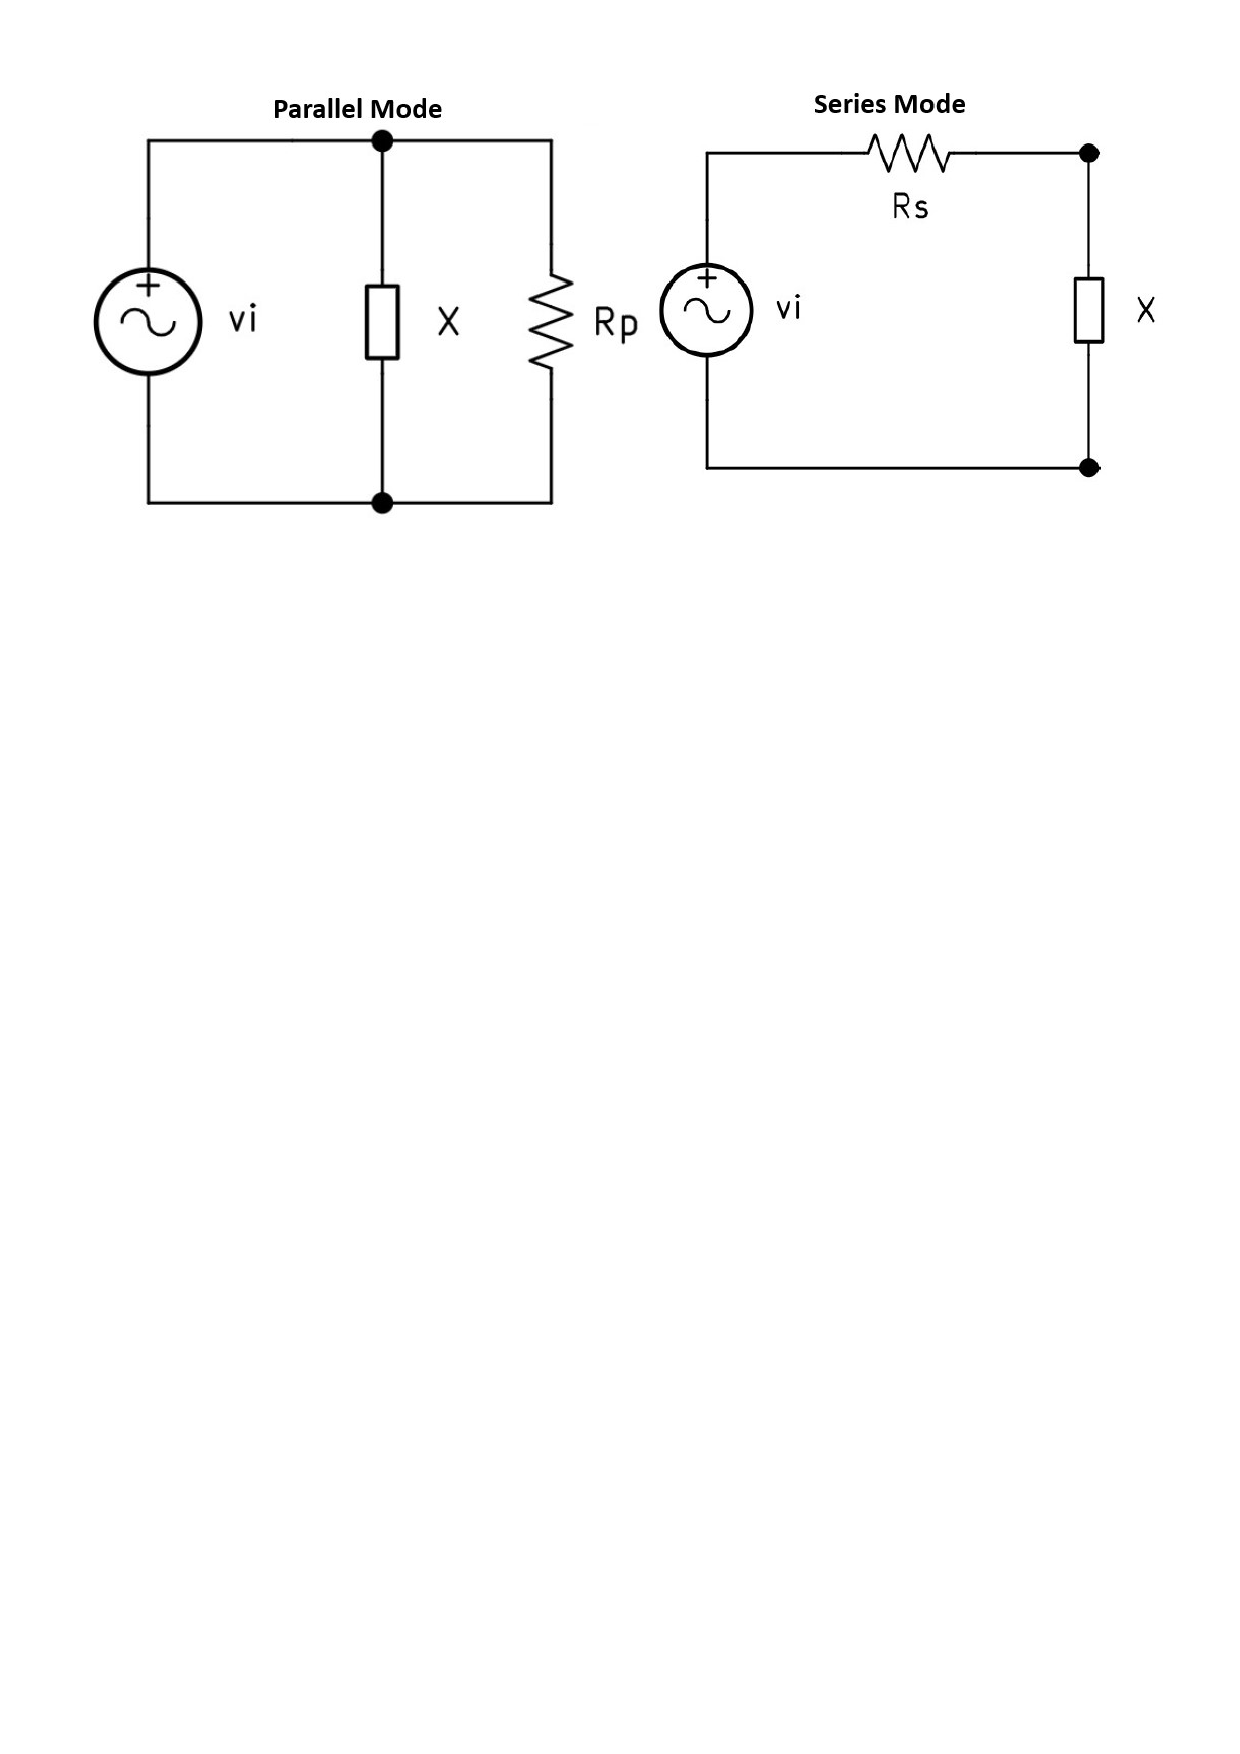
\includegraphics[clip, trim=0 550 0 0, width=0.8\textwidth]{Sections/4_TechnicalAnalysis/Figures/4_1_5_SeriesParallelMode.pdf}
    \caption{The two models that could be used for the DUT. The impedance measured can be fitted to either of them depending on the situation.}
    \label{fig:4_1_5_DUTXSeriesParallelMode}
\end{figure}

Assuming $\bar v$ and $\bar i$ from section \refq{sec:ImpedanceAnalysis} has been measured. The series model can be fitted to the impedance as $\bar Z =|\bar Z| \cdot \mathrm e^{\pm j\phi}$ where Rs and X will be the real and imaginary parts of the complex impedance as shown in eq \refq{eq:4_1_5_SeriesModel1}.

\begin{equation}\label{eq:4_1_5_SeriesModel1}
    \begin{split}
        R_s =& \Re(|\bar Z| \cdot \mathrm e^{\pm j\phi}) = |\bar Z| \cdot cos(\phi)\\
        X_s =& \Im(|\bar Z| \cdot \mathrm e^{\pm j\phi}) = \pm j\cdot |\bar Z| sin(\phi) 
    \end{split}
\end{equation}

These values in eq \refq{eq:4_1_5_SeriesModel1} can be used to fit the impedance to the series model shown on figure \refq{fig:4_1_5_DUTXSeriesParallelMode}. It may be desired to convert the series model to a parallel model as will be shown in subsection \refq{subsec:SeriesToParallel_conv}.

\subsubsection{Series to Parallel Conversion} \label{subsec:SeriesToParallel_conv}

A parallel model can also be used to represent the exact same impedance. To derive a set of equations that can convert a series impedance to a parallel impedance, the series impedance will first be analysed as a parallel admittance, as $Y_p = 1/Z_s$, as shown in figure \refq{fig:4_1_5_ParallelAdmittance}.

\begin{figure}[H]
    \centering
    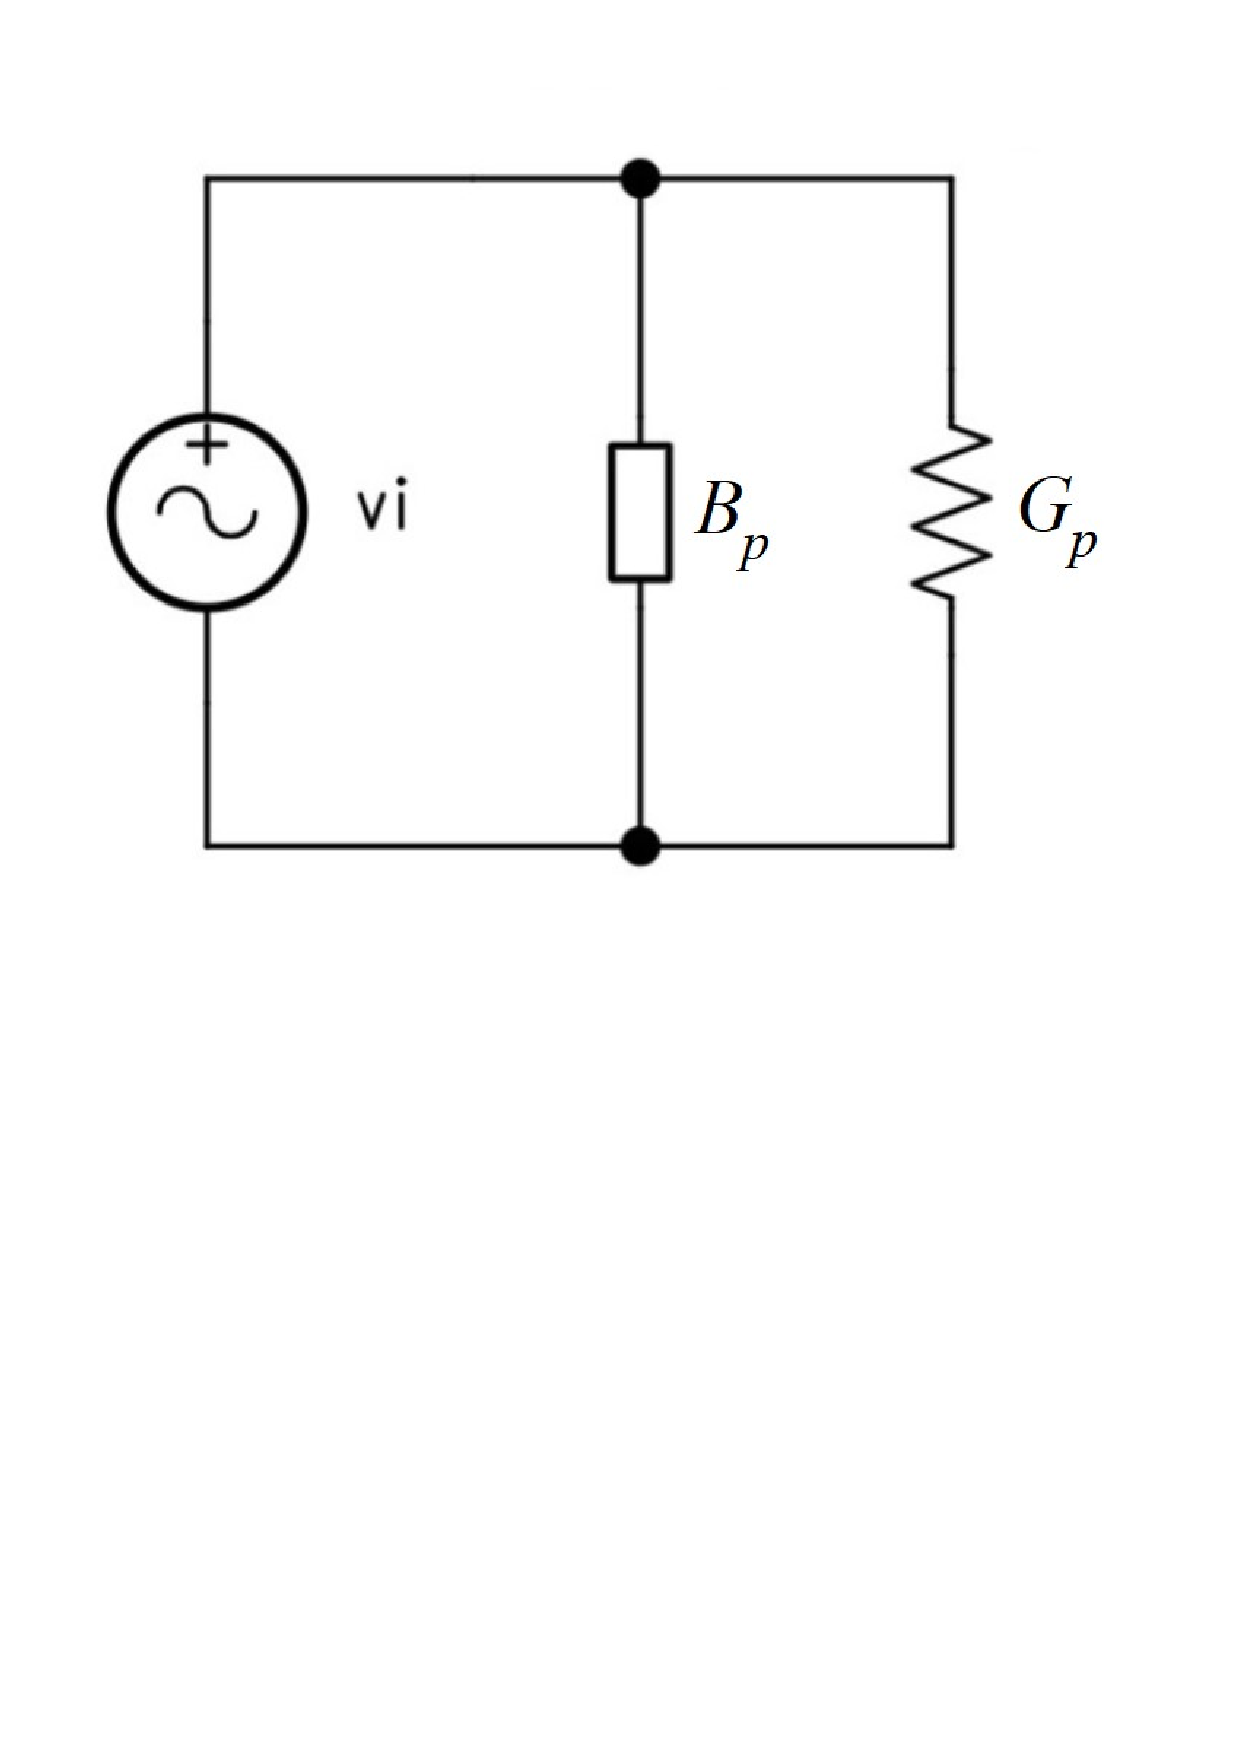
\includegraphics[clip, trim=0 400 0 0, width=0.5\textwidth]{Sections/4_TechnicalAnalysis/Figures/4_1_5_ParallelAdmittance.pdf}
    \caption{A circuit with a parallel admittance, $Y_p = 1/Z_s$}
    \label{fig:4_1_5_ParallelAdmittance}
\end{figure}

The admittance in figure \refq{fig:4_1_5_ParallelAdmittance} is given as $Y_p = G_p + jB_p$ and this admittance is the same as the reciprocal of impedance as shown in eq \refq{eq:4_1_5_ParallelModely1}.

\begin{equation}\label{eq:4_1_5_ParallelModely1}
    \begin{split}
        \frac{1}{Z_s}= Y_p = G_p +jB_p \\
    Y_p = \frac{1}{Z_s} = \frac{1}{R_s + jX_s} 
    \end{split}
\end{equation}

The expression for $1/Z_s$ in eq \refq{eq:4_1_5_ParallelModely1} will be complex conjugated as shown in eq \refq{eq:4_1_5_ParallelModely2}.

\begin{equation}\label{eq:4_1_5_ParallelModely2}
    \begin{split}
    \frac{1}{Z_s} = \frac{1(R_s - jX_s)}{(R_s + jX_s)(R_s - jX_s)}  \\
    \frac{1}{Z_s} = \frac{R_s - jX_s}{R_s^2+X_s^2} 
    \end{split}
\end{equation}

Comparing eq \refq{eq:4_1_5_ParallelModely2} to a complex admittance of the form $Y = G + jB$ the conductance and susceptance for the parallel admittance are as shown in eq
\begin{equation}\label{eq:4_1_5_ParallelModely3}
    \begin{split}
    G_p = \frac{R_s}{R_s^2 + X_s^2} \\
    B_p = -j\frac{X_s}{R_s^2 + X_s^2}
    \end{split}
\end{equation}

To preserve the \textbf{form} of the parallel circuit on figure \refq{fig:4_1_5_ParallelAdmittance} the real and imaginary components of the complex parallel admittance must be converted individually as shown in \refq{eq:4_1_5_ParallelModely4}.

\begin{equation}\label{eq:4_1_5_ParallelModely4}
    \begin{split}
    R_p = \frac{1}{G_p} = \frac{1}{\frac{R_s}{R_s^2 + X_s^2}} = \frac{R_s^2 + X_s^2}{R_s} \\
    X_p = \frac{1}{B_p} = \frac{1}{-j\frac{X_s}{R_s^2 + X_s^2}} = j\frac{R_s^2+X_s^2}{X_s}
    \end{split}
\end{equation}

A series impedance can be converted to a parallel impedance by using the expression from equation \refq{eq:4_1_5_ParallelModely4} and the full expression for the complex parallel impedance can be seen in eq \refq{eq:4_1_5_ParallelModely5}.
\begin{equation}\label{eq:4_1_5_ParallelModely5}
       Z_p = \frac{R_s^2 + X_s^2}{R_s} + j\frac{R_s^2+X_s^2}{X_s} 
\end{equation}

Eq \refq{eq:4_1_5_ParallelModely5} could be implemented in a microcontroller to do the conversion.

\subsubsection{Parallel to Series Conversion} \label{subsec:SeriesToParallel_conv2}

The parallel impedance, $Z_p = R_p + jX_p$, can be written in the form in equation \refq{eq:4_1_5_ParallelModelps1}. This form can be changed into a series impedance.

\begin{equation}\label{eq:4_1_5_ParallelModelps1}
        Z_p = \frac{R_p j X_p}{R_p + jX_p}
\end{equation}

To change the parallel impedance in eq \refq{eq:4_1_5_ParallelModelps1} into a series impedance the expression is first complex conjugated as shown in eq \refq{eq:4_1_5_ParallelModelps2}.

\begin{equation}\label{eq:4_1_5_ParallelModelps2}
    \begin{split}
    Z_p = \frac{(R_p j X_p)(R_p - jX_p)}{(R_p + jX_p)(R_p - jX_p)}  \\
    Z_p = \frac{R_p^2 jX_p + R_pX_p^2}{R_p^2+X_p^2}
    \end{split}
\end{equation}

To find the equivalent series impedance the real and imaginary parts of the parallel impedance in eq \refq{eq:4_1_5_ParallelModelps2} must be identified. This can be seen in eq \refq{eq:4_1_5_ParallelModelps3}.

\begin{equation}\label{eq:4_1_5_ParallelModelps3}
    \begin{split}
    R_s = \Re(Z_p) = \Re\left(\frac{R_p^2 jX_p + R_pX_p^2}{R_p^2+X_p^2}\right) = \frac{R_pX_p^2}{R_p^2+X_p^2}  \\
    X_s = \Im(Z_p)=\Im\left(\frac{R_p^2 jX_p + R_pX_p^2}{R_p^2+X_p^2}\right) = \frac{R_p^2X_p}{R_p^2+X_p^2}  \\
    \end{split}
\end{equation}

The expression for the real and imaginary parts in Eq \refq{eq:4_1_5_ParallelModelps3} can be used to find the impedance for the series equivalent impedance. This is shown in eq \refq{eq:4_1_5_ParallelModelps4}

\begin{equation}\label{eq:4_1_5_ParallelModelps4}
    Z_s = R_s + jX_s = \frac{R_pX_p^2}{R_p^2+X_p^2} + j\frac{R_p^2X_p}{R_p^2+X_p^2} 
\end{equation}

Eq \refq{eq:4_1_5_ParallelModelps4} can be programmed into a microcontroller to convert a parallel impedance to a series impedance.